\section{Appendix}

\begin{figure}[H]
    \centering
    \includegraphics[width=0.8\textwidth]{img/arcfaceframework.png}
    \caption{ArcFace training framework}
\end{figure}


\begin{figure}[H]
\centering
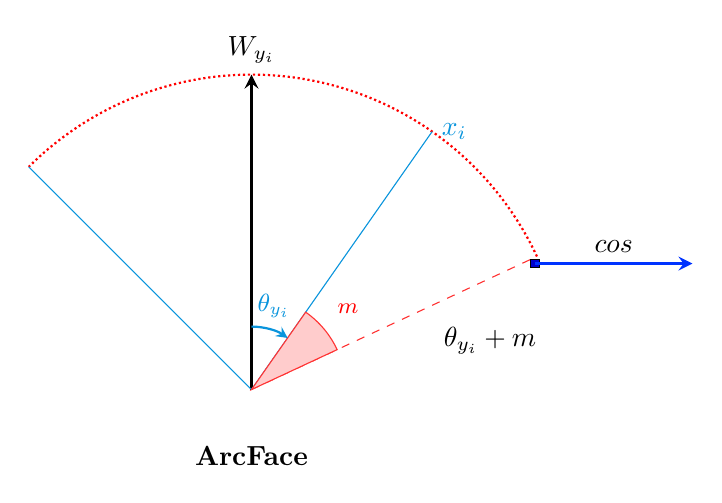
\begin{tikzpicture}[scale=2, >=stealth]
    % Origin
    \coordinate (O) at (0,0);
    \def\R{2} % Radius

    % --- W_yi Vector (Vertical) ---
    \draw[->, black, very thick] (O) -- (90:\R) node[above] {$W_{y_i}$};

    % --- Sector Arc (Red Dotted) ---
    % Spanning from roughly 135 to 25 degrees
    \draw[red, densely dotted, thick] (25:\R) arc (25:135:\R);

    % --- Left Radial Line (Blue) ---
    \draw[cyan!80!blue, thin] (O) -- (135:\R);

    % --- Right Radial Line (Blue) - representing x_i ---
    % Let's place x_i at 55 degrees (theta = 35)
    % And margin end at 25 degrees (m = 30)
    \def\angX{55}
    \def\angM{25}
    
    \draw[cyan!80!blue, thin] (O) -- (\angX:\R);
    \node[cyan!80!blue, right] at (\angX:\R) {$x_i$};
    
    % --- Red Dashed Line (Margin Boundary) ---
    \draw[red!80, dashed, thin] (O) -- (\angM:\R);
    
    % --- Margin Wedge (Red Filled) ---
    \draw[fill=red!20, draw=red!80] (O) -- (\angX:0.6) arc (\angX:\angM:0.6) -- cycle;
    \node[red, font=\footnotesize] at ({(\angX+\angM)/2}:0.8) {$m$};

    % --- Angle Theta_yi (Blue Arc) ---
    \draw[cyan!80!blue, thick, ->] (90:0.4) arc (90:\angX:0.4);
    \node[cyan!80!blue, font=\small] at (75:0.55) {$\theta_{y_i}$};


    % --- Label theta + m ---
    % Pointing to the dashed line area
    \node[right, black] at (15:1.2) {$\theta_{y_i} + m$};

    % --- Cosine Arrow on Right ---
    \coordinate (sq) at (1.8, 0.8);
    \node[draw, fill=blue!80!black, inner sep=1.5pt] (sq_node) at (sq) {};
    \draw[->, blue!80!cyan, very thick] (sq) -- ++(1.0, 0) node[midway, above, black] {$cos$};

    % --- Bottom Label ---
    \node[below, font=\bfseries] at (0,-0.3) {ArcFace};
\end{tikzpicture}
\caption{$x_i$ is embedding feature, $W_{y_i}$ is (sub-)center. Want: mininize distance of arc (geodesic distance) on hypersphere.}
\end{figure}

\begin{figure}[H]
    \centering
    \includegraphics[width=0.8\textwidth]{img/arcFacehiststartend.pdf}
    \caption{Target angle ($\theta$) distributions during ArcFace training}
\end{figure}

\begin{figure}[H]
    \centering
    \includegraphics[width=0.8\textwidth]{img/multicenter.png}
    \caption{Example of sub-classes after sub-center ArcFace}
\end{figure}

\begin{figure}[H]
    \centering
    \includegraphics[width=0.8\textwidth]{img/CASIAvariancedistribution2ECCV.pdf}
    \caption{Clean data isolation (dominant) after sub-center ArcFace}
\end{figure}


% \begin{figure}[H]
%     \centering
%     \includegraphics[width=0.8\textwidth]{img/IJBC.pdf}
%     \caption{ROC for test set IJB-C, trained with ResNet100 and dataset above}
% \end{figure}
